%

%\documentclass[utf8]{IEEEtran}
\documentclass[11pt]{article} 
%\documentclass[11pt,draftcls,journal,onecolumn]{../latexlib/ieee/IEEEtran}

% The preceding line is only needed to identify funding in the first footnote. If that is unneeded, please comment it out.
\usepackage{acronym}
\usepackage{algorithm}
\usepackage{algpseudocode}
\usepackage{amsmath}
\usepackage{amsmath, amssymb,longtable,dcolumn, nccmath}
\usepackage{balance}
\usepackage{bm}
%\usepackage[caption=false,font=footnotesize]{subfig}
\usepackage{cite}
\usepackage{colortbl}
\usepackage{csvsimple}
%\usepackage{enumitem} % also breaks things
\usepackage{fancyhdr}
%\usepackage{fixltx2e}
\usepackage{fullpage}
\usepackage{graphicx} 
%\usepackage{hyperref}  % Seems to break things
\usepackage{indentfirst}
\usepackage{multirow}
\usepackage{natbib}
\usepackage{pdfpages}
%\usepackage{stfloats}  % Written by Sigitas Tolusis
%\usepackage{subcaption}
%\usepackage{subfigure}
\usepackage{tabularx}
\usepackage{times}
\usepackage{units}
\usepackage{siunitx}

\usepackage{url}


% Requires sudo apt-get install texlive-publishers texlive-publishers-doc
\usepackage{IEEEtrantools}

% For Frontiers
\usepackage{url,hyperref,lineno,microtype,subcaption}
\usepackage[onehalfspacing]{setspace}

%\linenumbers

% Load this package last - for non-line-break hyphens (e.g., WAM-V)
% See https://tex.stackexchange.com/questions/103608/how-to-force-latex-not-to-break-the-line-after-a-hyphen
\usepackage[shortcuts]{extdash}

\author{\IEEEauthorblockN{Brian Bingham}
\IEEEauthorblockA{\textit{Naval Postgraduate School}\\
bbingham@nps.edu}}
  
% Affiliations should be keyed to the author's name with superscript numbers and be listed as follows: Laboratory, Institute, Department, Organization, City, State abbreviation (USA, Canada, Australia), and Country (without detailed address information such as city zip codes or street names).
% If one of the authors has a change of address, list the new address below the correspondence details using a superscript symbol and use the same symbol to indicate the author in the author list.
\begin{document}

% A few math shortcuts
% Stolen from Austratlian Center for Field Robotics
% Thanks Alex!
% bbing 24.02.03

% general global definitions
\newcommand{\Def}{\ {\buildrel \triangle\over =}\ }
\newcommand{\beq} {\begin{equation}}
\newcommand{\eeq} {\end{equation}}
%\newcommand{\beqn} {\begin{eqnarray}}
%\newcommand{\eeqn} {\end{eqnarray}}
%\newcommand{\E}[1] {\mbox{$ {\rm E} \{ #1 \}$ }}
\newcommand{\Es}[2] {\mbox{$ {\rm E}^{#1} \{ #2 \}$ }}
\newcommand{\Set}[1] {\mbox{$ \{ #1 \} $ }}
\newcommand{\Cal}[1] {\mbox{$ {\cal #1 } $}}
\newcommand{\PR}[1]  {\mbox{$ P(#1) $}}
\newcommand{\Pri}[2]  {\mbox{$ P_{#1}(#2) $}}
\newcommand{\PRi}[2]  {\mbox{$ P_{#1}(#2) $}}
\newcommand{\Pris}[3]  {\mbox{$ P_{#1}^{#2}(#3) $}}
\newcommand{\like}[1]  {\mbox{$ \Lambda(\bf #1) $}}
\newcommand{\likei}[2]  {\mbox{$ \Lambda_{#2}(\bf #1) $}}
\newcommand{\LL}[1]  {\mbox{$ l(#1) $}} % loglikelihood
\newcommand{\LLi}[2]  {\mbox{$ l_{#1}(#2) $}} %loglikelihood
\newcommand{\EN}[1]  {\mbox{$ H(#1) $}} % entropy
\newcommand{\ENi}[2]  {\mbox{$ H_{#1}(#2) $}} % entropy
\newcommand{\mEN}[1]  {\mbox{$ \overline{H}(#1) $}} % mean entropy
\newcommand{\MI}[1]  {\mbox{$ I(#1) $}}  %mutual information
\newcommand{\est}[1]  {\mbox{$\hat{\bf #1}$}}
\newcommand{\estk}[2]  {\mbox{$\hat{\bf #1}(#2)$}}
\newcommand{\D}[1]    {\mbox{${\rm d} {#1}$}}
\newcommand{\mean}[1] {\mbox{$\overline{ #1}$}}
\newcommand{\Det}[1] {\mbox{$\mid {#1} \mid $}}
\newcommand{\One}      {\mbox{${\bf 1}$}}
\newcommand{\Zero}      {\mbox{${\bf 0}$}}
\newcommand{\grad}[1] {\mbox{${\bf\nabla} #1$}}
%\newcommand{\J}[3] {\mbox{${\bf\nabla}{\bf #1}_{\bf #2}(#3)$}}
\newcommand{\Jt}[3] {\mbox{${\bf\nabla}^T{\bf #1}_{\bf #2}(#3)$}}
\newcommand{\pdf}{{\it pdf\ }}
\newcommand{\dxt}[2]  {\mbox{$\dot{\bf #1}( #2)$}}
% defining different types of vectors
% first those with no time subscripts
\renewcommand{\V}[1] {\mbox{${\bf #1}$}}
\newcommand{\Vt}[1] {\mbox{${\bf #1}^T$}}
\newcommand{\Vin}[1] {\mbox{${\bf #1}^{-1}$}}
\newcommand{\Vgin}[1] {\mbox{${\bf #1}^{\dagger}$}}
\newcommand{\Vi}[2] {\mbox{${\bf #1}_{#2}$}}
\newcommand{\Vs}[2] {\mbox{${\bf #1}^{#2}$}}
\newcommand{\Vis}[3] {\mbox{${\bf #1}_{#2}^{#3}$}}
\newcommand{\Vit}[2] {\mbox{${\bf #1}_{#2}^T$}}
\newcommand{\Vini}[2] {\mbox{${\bf #1}_{#2}^{-1}$}}
\newcommand{\Vgini}[2] {\mbox{${\bf #1}^{\dagger}$}}

% next those with time subscript k (very common)
\newcommand{\Vk}[1] {\mbox{${\bf #1}(k)$}}
\newcommand{\Vkt}[1] {\mbox{${\bf #1}^T(k)$}}
\newcommand{\Vkin}[1] {\mbox{${\bf #1}^{-1}(k)$}}
\newcommand{\Vkgin}[1] {\mbox{${\bf #1}^{\dagger}(k)$}}
\newcommand{\Vki}[2] {\mbox{${\bf #1}_{#2}(k)$}}
\newcommand{\Vks}[2] {\mbox{${\bf #1}^{#2}(k)$}}
\newcommand{\Vkis}[3] {\mbox{${\bf #1}_{#2}^{#3}(k)$}}
\newcommand{\Vkit}[2] {\mbox{${\bf #1}_{#2}^T(k)$}}
\newcommand{\Vkini}[2] {\mbox{${\bf #1}_{#2}^{-1}(k)$}}
\newcommand{\Vkgini}[2] {\mbox{${\bf #1}^{\dagger}_{#2}(k)$}}
\newcommand{\tVk}[1] {\mbox{$\tilde{\bf #1}(k)$}}
\newcommand{\tVki}[2] {\mbox{$\tilde{\bf #1}_{#2}(k)$}}

% now those with general purpose time subscripts
%\newcommand{\Vec}[2] {\mbox{${\bf #1}(#2)$}}
\newcommand{\Vect}[2] {\mbox{${\bf #1}^T(#2)$}}
\newcommand{\Vecin}[2] {\mbox{${\bf #1}^{-1}(#2)$}}
\newcommand{\Veci}[3] {\mbox{${\bf #1}_{#2}(#3)$}}
\newcommand{\Vecit}[3] {\mbox{${\bf #1}_{#2}^T(#3)$}}
\newcommand{\Vecini}[3] {\mbox{${\bf #1}_{#2}^{-1}(#3)$}}
\newcommand{\Vecgin}[2] {\mbox{${\bf #1}^{\dagger}(#2)$}}
\newcommand{\Vecgini}[3] {\mbox{${\bf #1}^{\dagger}_{#2}(#3)$}}

% special symbols used very commonly
% state estimates of different sorts
\newcommand{\x}[2] {\mbox{$\hat{\bf x}( #1 \mid #2)$}}
\newcommand{\ix}[3] {\mbox{$\hat{\bf x}_{#1}( #2 \mid #3)$}}
\newcommand{\tx}[2] {\mbox{$\tilde{\bf x}( #1 \mid #2 )$}}
\newcommand{\txi}[3] {\mbox{$\tilde{\bf x}_{#1}( #2 \mid #3 )$}}
\newcommand{\z}[2] {\mbox{$\hat{\bf z}( #1 \mid #2)$}}
\newcommand{\tz}[2] {\mbox{$\tilde{\bf z}( #1 \mid #2)$}}
\newcommand{\tzt}[2] {\mbox{$\tilde{\bf z}^T( #1 \mid #2)$}}
\newcommand{\zi}[3] {\mbox{$\hat{\bf z}_{#1}( #2 \mid #3)$}}
\newcommand{\di}[3] {\mbox{$\hat{\bf \delta}_{#1}( #2 \mid #3)$}}

% variances of different sorts
\newcommand{\var}[2] {\mbox{${\bf P}( #1 \mid #2)$}}
\newcommand{\varin}[2] {\mbox{${\bf P}^{-1}( #1 \mid #2)$}}
\newcommand{\tvar}[2] {\mbox{$\tilde{\bf P}( #1 \mid #2)$}}
\newcommand{\tvarin}[2] {\mbox{$\tilde{\bf P}^{-1}( #1 \mid #2)$}}
\newcommand{\vari}[3] {\mbox{${\bf P}_{#1}( #2 \mid #3)$}}
\newcommand{\varini}[3] {\mbox{${\bf P}^{-1}_{#1}( #2 \mid #3)$}}
\newcommand{\tvari}[3] {\mbox{$\tilde{\bf P}_{#1}( #2 \mid #3)$}}
\newcommand{\tvarini}[3] {\mbox{$\tilde{\bf P}^{-1}_{#1}( #2 \mid #3)$}}

% information states and variances
\newcommand{\y}[2] {\mbox{$\hat{\bf y}( #1 \mid #2)$}}
\newcommand{\ty}[2] {\mbox{$\tilde{\bf y}( #1 \mid #2)$}}
\newcommand{\yi}[3] {\mbox{$\hat{\bf y}_{#1}( #2 \mid #3)$}}
\newcommand{\tyi}[3] {\mbox{$\tilde{\bf y}_{#1}( #2 \mid #3)$}}
\newcommand{\Y}[2] {\mbox{${\bf Y}( #1 \mid #2)$}}
\newcommand{\Yin}[2] {\mbox{${\bf Y}^{-1}( #1 \mid #2)$}}
\newcommand{\tY}[2] {\mbox{$\tilde{\bf Y}( #1 \mid #2)$}}
\newcommand{\Yi}[3] {\mbox{${\bf Y}_{#1}( #2 \mid #3)$}}
\newcommand{\Yini}[3] {\mbox{${\bf Y}_{#1}^{-1}( #2 \mid #3)$}}
\newcommand{\tYi}[3] {\mbox{$\tilde{\bf Y}_{#1}( #2 \mid #3)$}}
\newcommand{\info}[1] {\mbox{${\bf i}( #1)$}}
\newcommand{\Info}[1] {\mbox{${\bf I}( #1)$}}
\newcommand{\infoi}[2] {\mbox{${\bf i}_{#1}( #2)$}}
\newcommand{\infois}[3] {\mbox{${\bf i}_{#1}^{#2}(#3)$}}
\newcommand{\Infoi}[2] {\mbox{${\bf I}_{#1}( #2)$}}
\newcommand{\tInfoi}[2] {\mbox{$\tilde{\bf I}_{#1}( #2)$}}
\newcommand{\Infoini}[2] {\mbox{${\bf I}^{\dagger}_{#1}( #2)$}}
\newcommand{\Prop}[2] {\mbox{${\bf L}( #1 \mid #2)$}}
\newcommand{\Propi}[3] {\mbox{${\bf L}_{#1}( #2 \mid #3)$}}
\newcommand{\Z}[2] {\mbox{${\cal Z}^{#1}_{#2}$}}

% spurious ones
\newcommand{\maybe}{\ {\buildrel ?\over =}\ } %chapter 4
\newcommand{\svd} {\mbox{$\dagger$}} % chapter 4
\newcommand{\dnoise} {\mbox{$\delta d$}} % chapter 6 and 7
\newcommand{\unoise} {\mbox{$\delta u$}} % chapter 6
%\newcommand{\ns}[1] {\mbox{$ #1$}} % chapter 6
\newcommand{\vs} {\vspace{0.17in}}
\newcommand{\svs} {\vspace{0.17cm}}
\newcommand{\vsf} {\vspace{0.4in}}
\newcommand{\vsff} {\vspace{1in}}
\newcommand{\veqns} {\vspace{-0.15in}}
\newcommand{\veqn} {\vspace{-0.12in}}
\newcommand{\sveqn} {\vspace{-0.06in}}
%\newcommand{\bc}{\begin{center}}
%\newcommand{\ec}{\end{center}}
%\newcommand{\bi}{\begin{itemize}}
%\newcommand{\ei}{\end{itemize}}
%\newcommand{\be}{\begin{enumerate}}
%\newcommand{\ee}{\end{enumerate}}
\newcommand{\Quote}{\parbox[t]{12.5cm}}
\newtheorem{example}{Example}


% set the figure default size
\newcommand{\SF}{0.7}
\newcommand{\SFb}{0.45}
\newcommand{\SFPic}{0.45}
\newcommand{\SFPlot}{0.45}
\newcommand{\SFc}{0.45}
% Just a lazy way of setting the figure width (percentage of text width)
% 0.7 works well for 1 column
% 0.4 works well for 2 column
\newcommand{\FigWidth}{\SFb}

\newcommand{\figref}[1] {Fig.~\ref{#1}}

% To prevent line break
\newcommand{\wamv}{WAM\=/V}

% Use this one for the draft version
\newcommand{\scaleOneTwo}[2] {\scalebox{#1}}
% Use this one for the two column version
%\newcommand{\scaleOneTwo}[2] {\scalebox{#2}}

% Graphics for this paper
\graphicspath{{./images/}{./src/}}

\title{VRX Wind}
\author{Brian Bingham \\ Naval Postgraduate School}


% make the title area
\maketitle


\section{Environment Modeling}
A key aspect of extending the Gazebo robotics simulator to support ocean robotics is the ability to represent the influence of the ocean environment on the robotic system.  For USV applications the most important environmental influences are waves and wind.

VRX uses a model-based approach where the models are based on spectral representations of the stochastic wave and wind environments.  Empirical environmental models are described as power spectral density (PSD) representations.  We adopt spectral representation methods \citep{shinozuka91simulation} to generate time series realizations of the stochastic process with the prescribed PSD.  Because wind and wave environments are often characterized by power spectra, this approach allows simulations to be tied directly to standard ocean environments with mature descriptions from oceanography.


\subsection{Wind Modeling}\label{s:wind_model}
Wind is a significant disturbance for objects at the sea surface. We consider the total wind speed $V_w(t)$ consisting of the sum of the constant mean wind speed ($\bar{v}$) and stochastic, zero-mean, variable wind speed ($v_g(t)$) due to turbulence and gusting, i.e., $V_w(t)=\bar{v}+v_g(t)$.

Spectral representations of ocean wind environments are common and generally model the variable component of wind speed as a wide-sense stationary, Gaussian stochastic process.  Typical models of wind over water include \citet{harris71nature}, \citet{forristall88wind} and \citet{ochi13wind}. \citet{cole18reactive} showed that the Forristall and Ochi and Shin models are in agreement, while the Harris model underestimates the spectral content.  While the implementation is not specific to any one spectral model of stochastic wind, for illustration purposes we use the Forristall wind spectra.  The form of the one-sided spectra is \citet{olesen84modelling} blunt model for micrometeorology, where Forristall showed that normalizing the one-sided spectrum by the variance ($\sigma$) produced improved experimental agreement:
\begin{equation}
  \widetilde{S}_f(f) = \frac{S_f(f)\,f}{\sigma^2}  = \frac{ A f^*}{( 1 + B f^*)^{5/3}}.
    \label{e:forristall}
    \end{equation}
    In this dimensionless form $f$ is the oscillation frequency in \unit[]{Hz} and $f^*$ is the standard nondimenstional frequency from atmospheric boundary layer studies,
\begin{equation}
  f^* = \frac{f \, z}{\bar{v}(z)},
\end{equation}
where $z$ is the height and $\bar{v}(z)$ is the mean wind speed as a function of height. The constants $A$ and $B$ are chosen to fit specific observational data.  We use the mean coefficients from of $A=42.0$ and $B=63.0$, as reported by \citet{forristall88wind}  These values satisfy the constraint $A=(2/3)B$, necessary so that the variance of the stochastic process is $\sigma^2$, i.e.,
\begin{equation}
  \int_0^{\infty} S_f(f) df = \sigma^2.
\end{equation}
The Forristall normalized spectrum is illustrated in Figure~\ref{f:forristall_norm}.   The peak of the spectrum (\ref{e:forristall}) occurs at
\begin{equation}
f^*_p = \frac{3}{2B}.
\end{equation}
%so for a height of $z=\unit[10]{m}$ the dimensional peak frequency increases linearly with wind velocity,
%\begin{equation}
%f_p = \frac{3}{2Bz}\bar{v}_{10}.
%\end{equation}
\begin{figure}[h!]
  \centering
  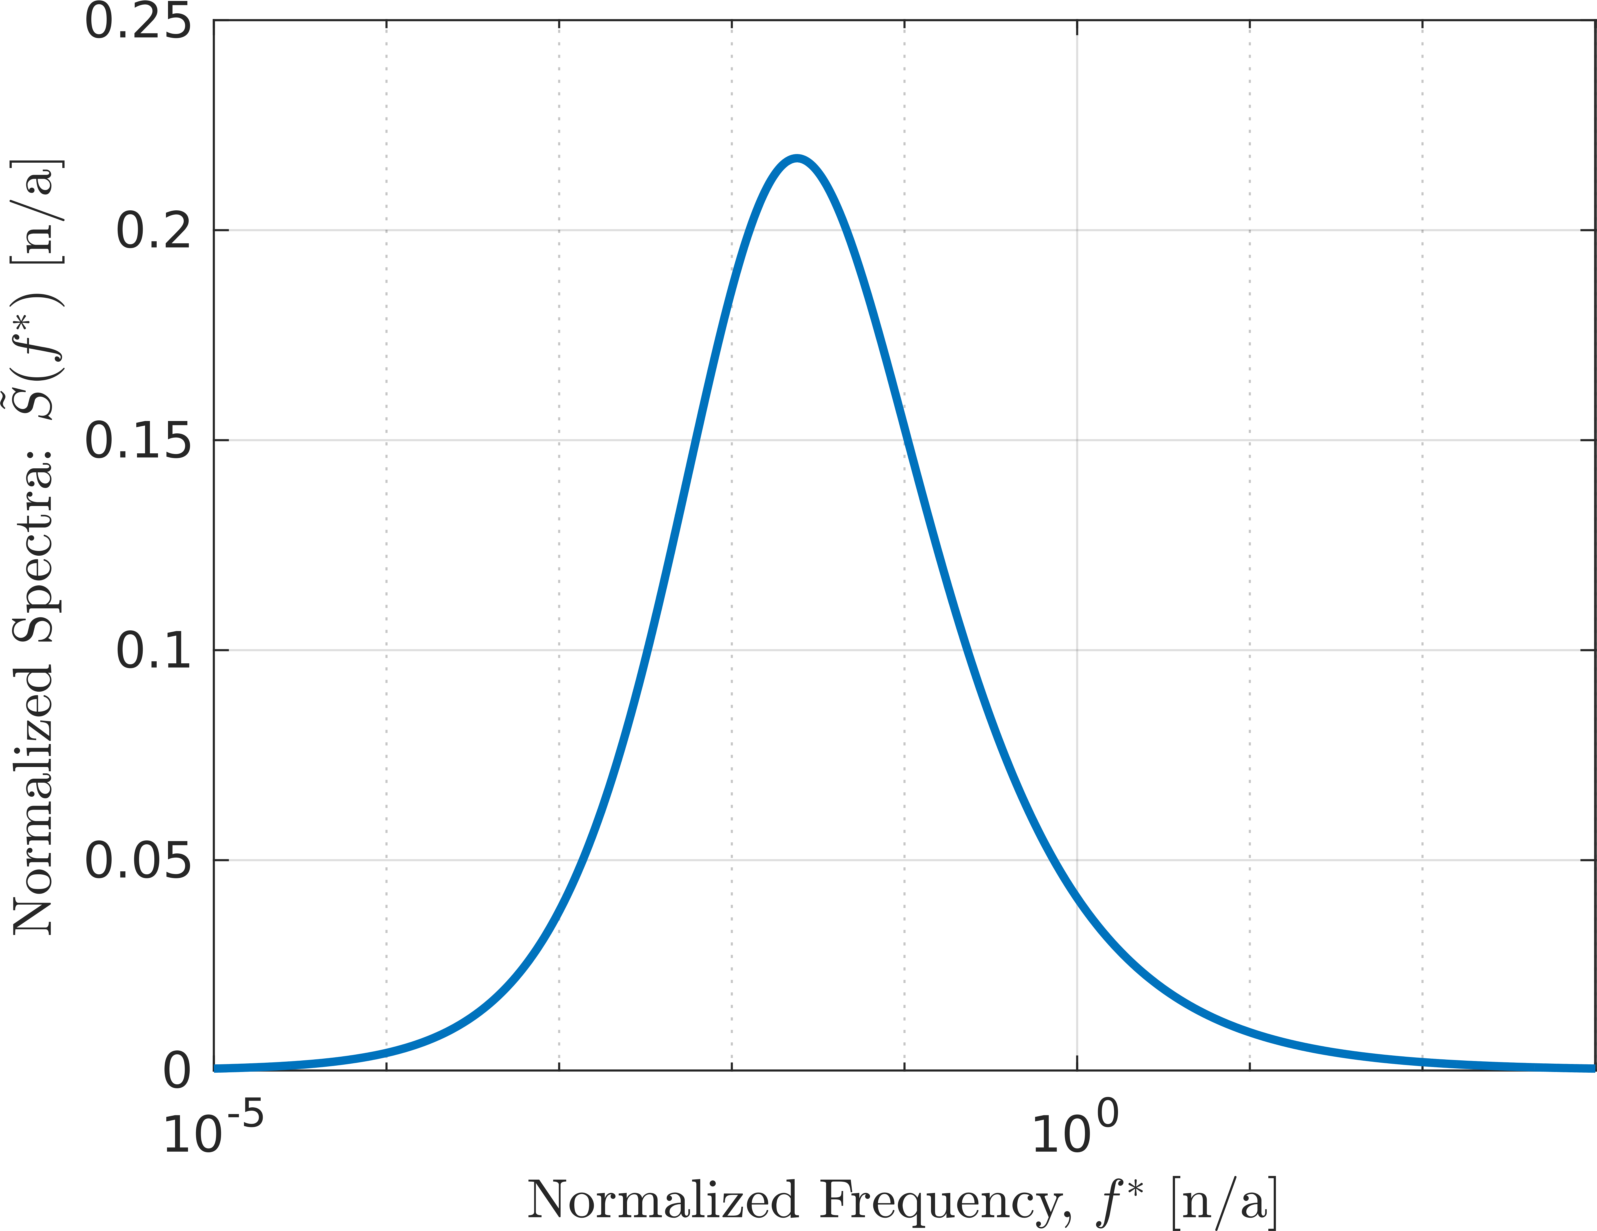
\includegraphics[width=\SFc\textwidth]{forristall_norm.png}
  \caption{Forristall normalized spectrum.}
  \label{f:forristall_norm}
\end{figure}

For generating physically meaningful wind time series simulations it is necessary to take into account the physical dimesions of the spectra.  We consider a constant height of $z=\unit[10]{m}$ and mean wind velocity at that height $\bar{v}(z=10)=\bar{v}_{10}$.  Figure~\ref{f:forristall_dim} illustrates how mean wind speed affects the generated spectra. 
\begin{figure}[hbt!]
  \centering
  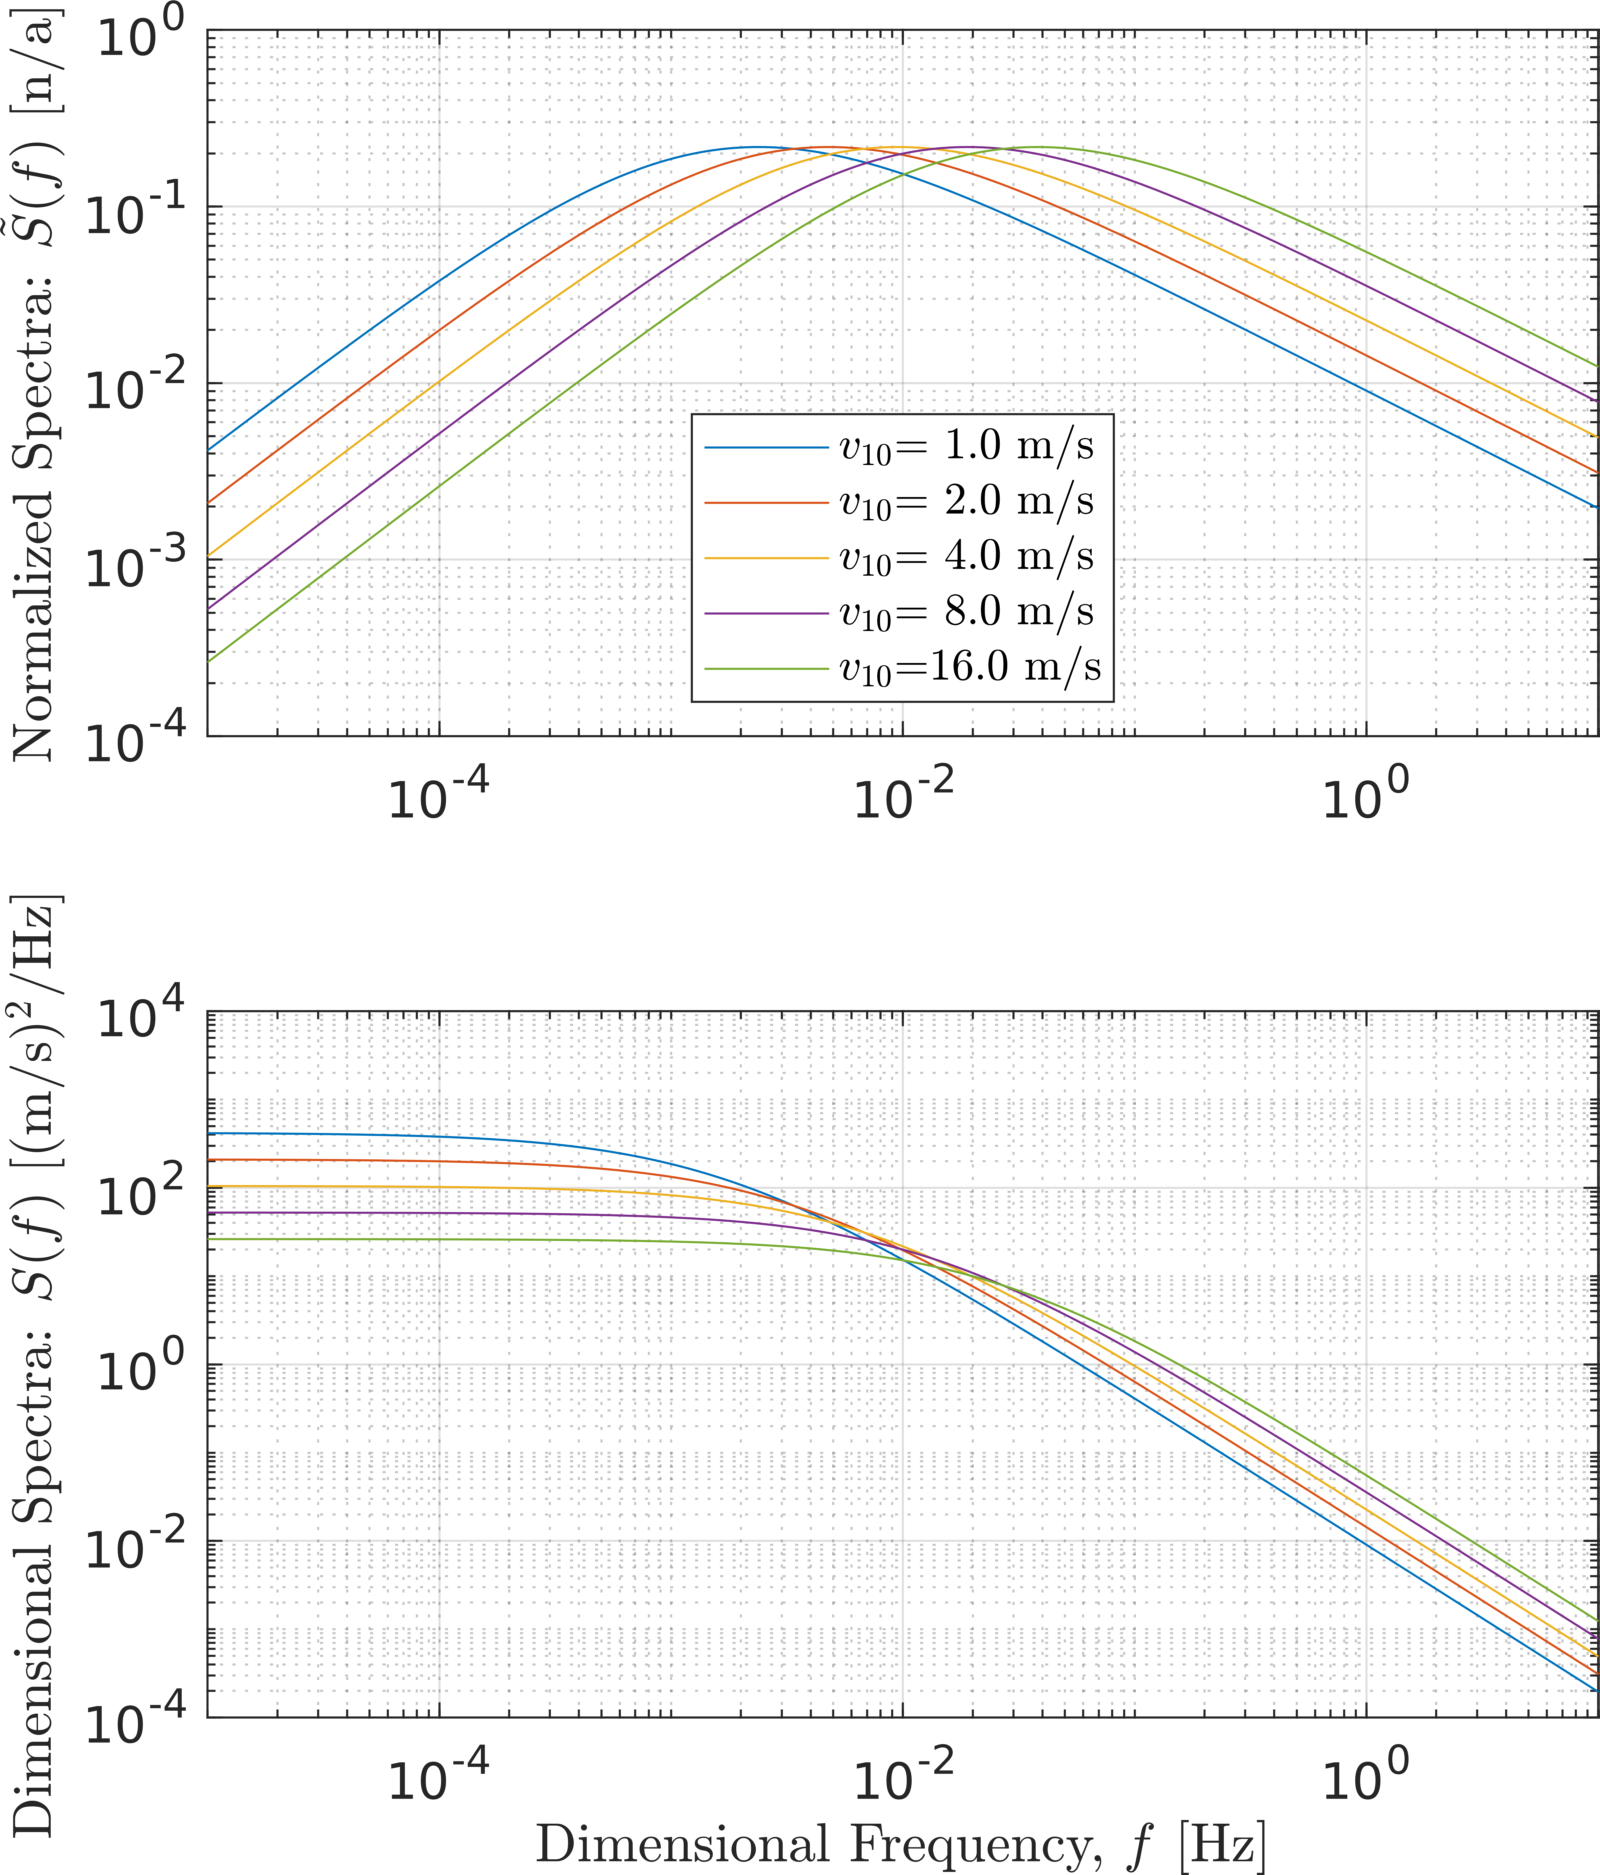
\includegraphics[width=\SFc\textwidth]{forristall_dim.png}
  \caption{Dimensional Forristall spectra with unit variance. }
  \label{f:forristall_dim}
\end{figure}
The cutoff frequency $f_c$ for the dimensional spectra is the frequency for which $S_f(f_c) = 0.5 S_f(0)$.  In dimensionless and dimensional forms, the cutoff frequency is
\begin{IEEEeqnarray}{rCl}\IEEEyesnumber\label{e:cutoff}
  f^*_c & = & \frac{2^{3/5}-1}{B} \\
  f_c & = & \frac{(2^{3/5}-1)\bar{v}(z)}{B\,z} \\
      & = & (\num{8.19e-4}) \, \bar{v}_{10} %\; \mathrm{Hz}.
  \end{IEEEeqnarray}

\subsubsection{Wind speed variance}
In the Forristall model the variance of the wind speed is not a simple function of the mean wind speed.  The ratio of the variance to the friction velocity ($v_*$) can be approximated as
\begin{equation}
\frac{\sigma}{v_*} = 3.0 w
\label{e:sigratio}
\end{equation}
where $w$ is determined from the predicted ocean significant wave height $H_n$ and the observed significant wave height $H_s$ as
\begin{equation}
w = 1 + \frac{H_s-H_n}{2 H_n}.
\label{e:wavefactor}
\end{equation}
For the purposes of this example, we consider a developed sea where $H_s=H_n$.

The friction velocity is determined by using the logarithmic boundary layer mean velocity profile
\begin{equation}
\bar{v}(z) = \frac{v_*}{\kappa}\ln{\left(\frac{z}{z_0}\right)}
\label{e:profile}
\end{equation}
where the von Karman's constant is $\kappa=0.41$ and $z_0$ is the sea surface roughness.  It is common to re-write (\ref{e:profile}) at a reference altitude of $z=\unit[10]{m}$ and solve for the friction velocity
\begin{equation}
v_* = \frac{\kappa \, \bar{v}(z=10)}{\ln(z=10/z_0)} = \frac{\kappa \, \bar{v}_{10}}{\ln(10/z_0)}.
\label{e:profile10}
\end{equation}
Multiple models of the relationship between sea surface roughness ($z_0$) and friction velocity ($v_*$) are available.  Based on dimensional analysis \citet{charnock55wind} proposed 
\begin{equation}
\frac{z_0 g }{v_*^2} = \alpha
\label{e:charnock}
\end{equation}
where $g$ is the acceleration of gravity; $\alpha = [0.013, 0.0185]$ has been found to be consistent with empirical wind profiles over the ocean \citep{garratt77review,toba90wave}.  %Alternatively this relationship can be considered to be a function of the degree of wave development, or wave age,
%\begin{equation}
%\frac{z_0 g }{v_*^2} = \mathsf{f} (c_p/v_*)
%\label{e:waveage}
%\end{equation}
%where $c_p$ is the phase velocity of the dominant wave and $c_p/v_*$ describes wave age \citep{myrhaung09effect}.  An example of the functional relationship for (\ref{e:waveage}) is provided in \citep{volkov01dependence}.

Without loss of generality, we numerically solve for $V_{*}$ by combining (\ref{e:profile10}) and (\ref{e:charnock}) with $\alpha= 0.0144$ for values of $v_{10} = [4, 21]\unit[]{m/s}$ \citep{garratt77review}.  The resulting values are illustrated in Figure~\ref{f:wind_consts}.
\begin{figure}[hbt!]
  \centering
  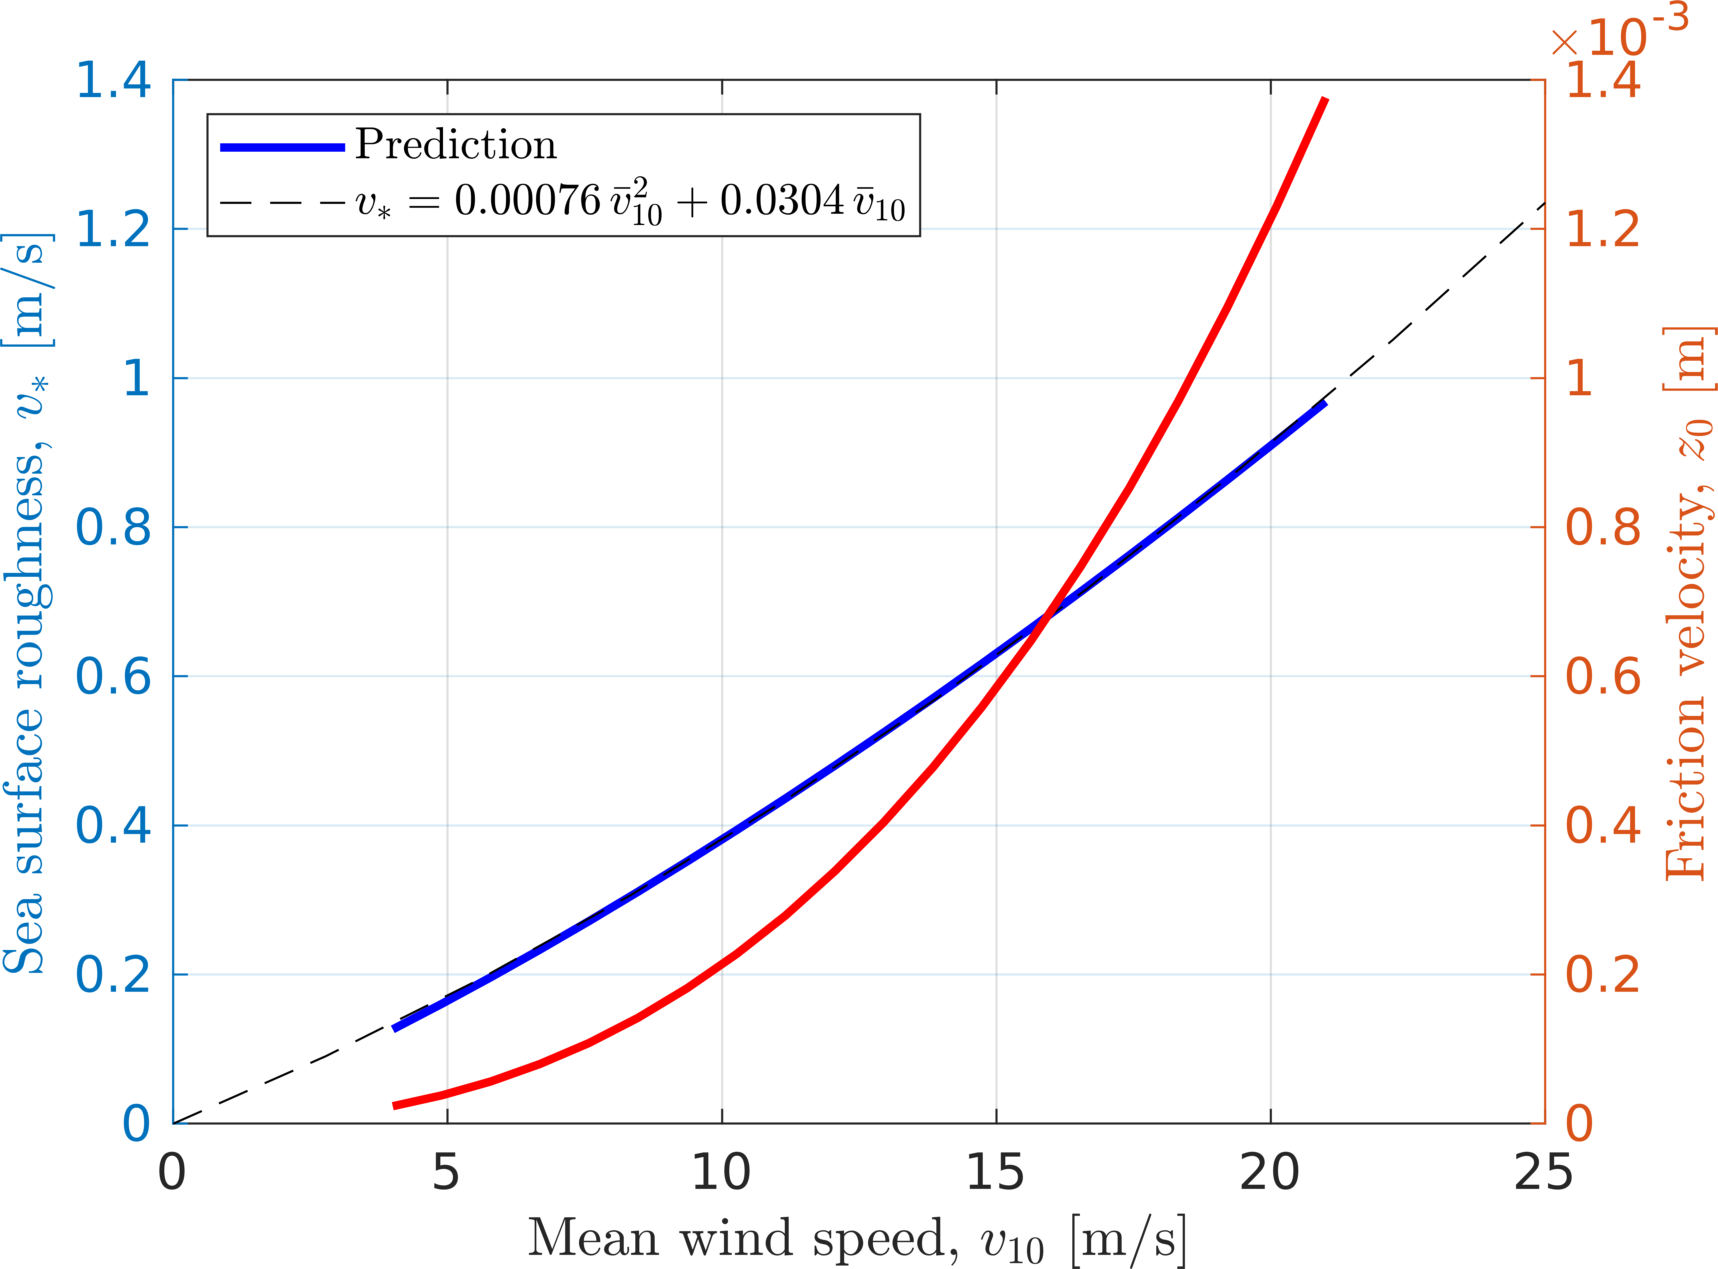
\includegraphics[width=\SFc\textwidth]{wind_consts.png}
  \caption{Sea surface roughness and friction velocity as a function of mean wind speed.}
  \label{f:wind_consts}
\end{figure}
To simplify the implementation, we fit a quadratic polynomial to the sea surface roughness prediction via nonlinear regression, enforcing that the y-intercept be zero.  The resulting relationship, also shown in Figure~\ref{f:wind_consts}, is
\begin{equation}
v_* = 0.00076 \, \bar{v}_{10}^2 + 0.0304 \, \bar{v}_{10}
\label{e:fit}
\end{equation}
which allows expression of the wind speed variance as a function of mean wind speed,
\begin{equation}
\sigma^2 = \left[ 3 \, w (0.00076 \, \bar{v}_{10}^2 + 0.0304 \, \bar{v}_{10})\right]^2.
\label{e:fit2}
\end{equation}
Substituting (\ref{e:forristall}) and the constants described above into (\ref{e:fit2})  allows us to express the dimensional Forristall spectrum for wind speed at $z=\unit[10.0]{m}$ altitude as a function of only the mean wind speed,
\begin{multline}
S_f(f) =  \left[ 3 \, (0.00076 \, \bar{v}_{10}^2 + 0.0304 \, \bar{v}_{10})\right]^2 \\
\frac{(42.0)10.0/\bar{v}_{10}}{\left(1+\frac{63.0 (10.0) f}{\bar{v}_{10}}\right)^{5/3}}.
\label{e:dimensional}
\end{multline}

\subsubsection{Generating Wind Time Series}
The wind model is described by the PSD in (\ref{e:dimensional}) which allows us to generate sample functions of the underlying stochastic process using a summation of cosines approach similar to the implementation of the Gerstner waves.  The combined turbulence and gusting wind speed is expressed as
\begin{equation}
  v_g(t) = \sqrt{2} \sum_{n=0}^{M-1} A_n \cos(\omega_n t + \phi_n)
  \label{e:sumcosines}
\end{equation}
where
\begin{IEEEeqnarray}{C}
\IEEEyesnumber\label{e:sim2} \IEEEyessubnumber*
A_n = \left(\frac{1}{2 \pi} S_{f}(f_n = \omega_n / (2 \pi)) \Delta \omega\right)^{1/2},  \label{e:an} \\
\omega_n = n \Delta \omega, \; n=0,1,2,...,N-1 \label{e:lrs2}\\
\Delta \omega = \omega_u / M.
\end{IEEEeqnarray}
The frequency sampling is $\Delta\omega$, the upper cut-off frequency, $\omega_u$, is the frequency beyond which the PSD may be assumed to be zero, $\phi_0, \phi_1, ... , \phi_{M-1}$ are random phase angles distributed uniformly over the interval $[0,2\pi)$.  Note the factor of $1/(2\pi)$ in (\ref{e:an}) is necessary to maintain the integral relationship between the spectrum and the variance of the underlying stochastic process, i.e.,
\begin{IEEEeqnarray}{rcl}
\IEEEyesnumber\label{e:freq} \IEEEyessubnumber*
E[v_g^2(t)] & = & \sigma_{v_g}^2 \\
& = &\int_{0}^{\infty}S_{f}(f)df \\
& = &\frac{1}{2\pi}\int_{0}^{\infty}S_{f}(f=\frac{\omega}{2\pi}) d\omega \\
& \leq & \frac{1}{2} \left( \frac{2 \pi}{\Delta \omega} \right) \frac{1}{M}.
\end{IEEEeqnarray}
The condition
\begin{equation}
  A_0 = 0 \; \mathrm{or} \; S_{f}(\omega_0=0)=0
  \label{e:an0}
\end{equation}
is necessary and must be forced if $S_{yy}(0)\neq 0$.  The resulting simulated time series is periodic with period
\begin{equation}
  \label{e:T0}
  T_0 = \frac{2\pi}{\Delta \omega}.
\end{equation}

By combining (\ref{e:dimensional}), (\ref{e:sumcosines}) and (\ref{e:sim2}) we are able to generate a physically relevant time series realization, $v_g$, of the variable wind speed stochastic process described by the Forristall wind spectrum.  For wind at $z=0$ and a fully developed sea ($H_s=H_n$) this time series is solely a function of mean wind speed, $\bar{v}=v_{10}$. The example in Figure~\ref{f:forristall} illustrates the results for three different mean wind speeds.
\begin{figure}[h!]
  \centering
  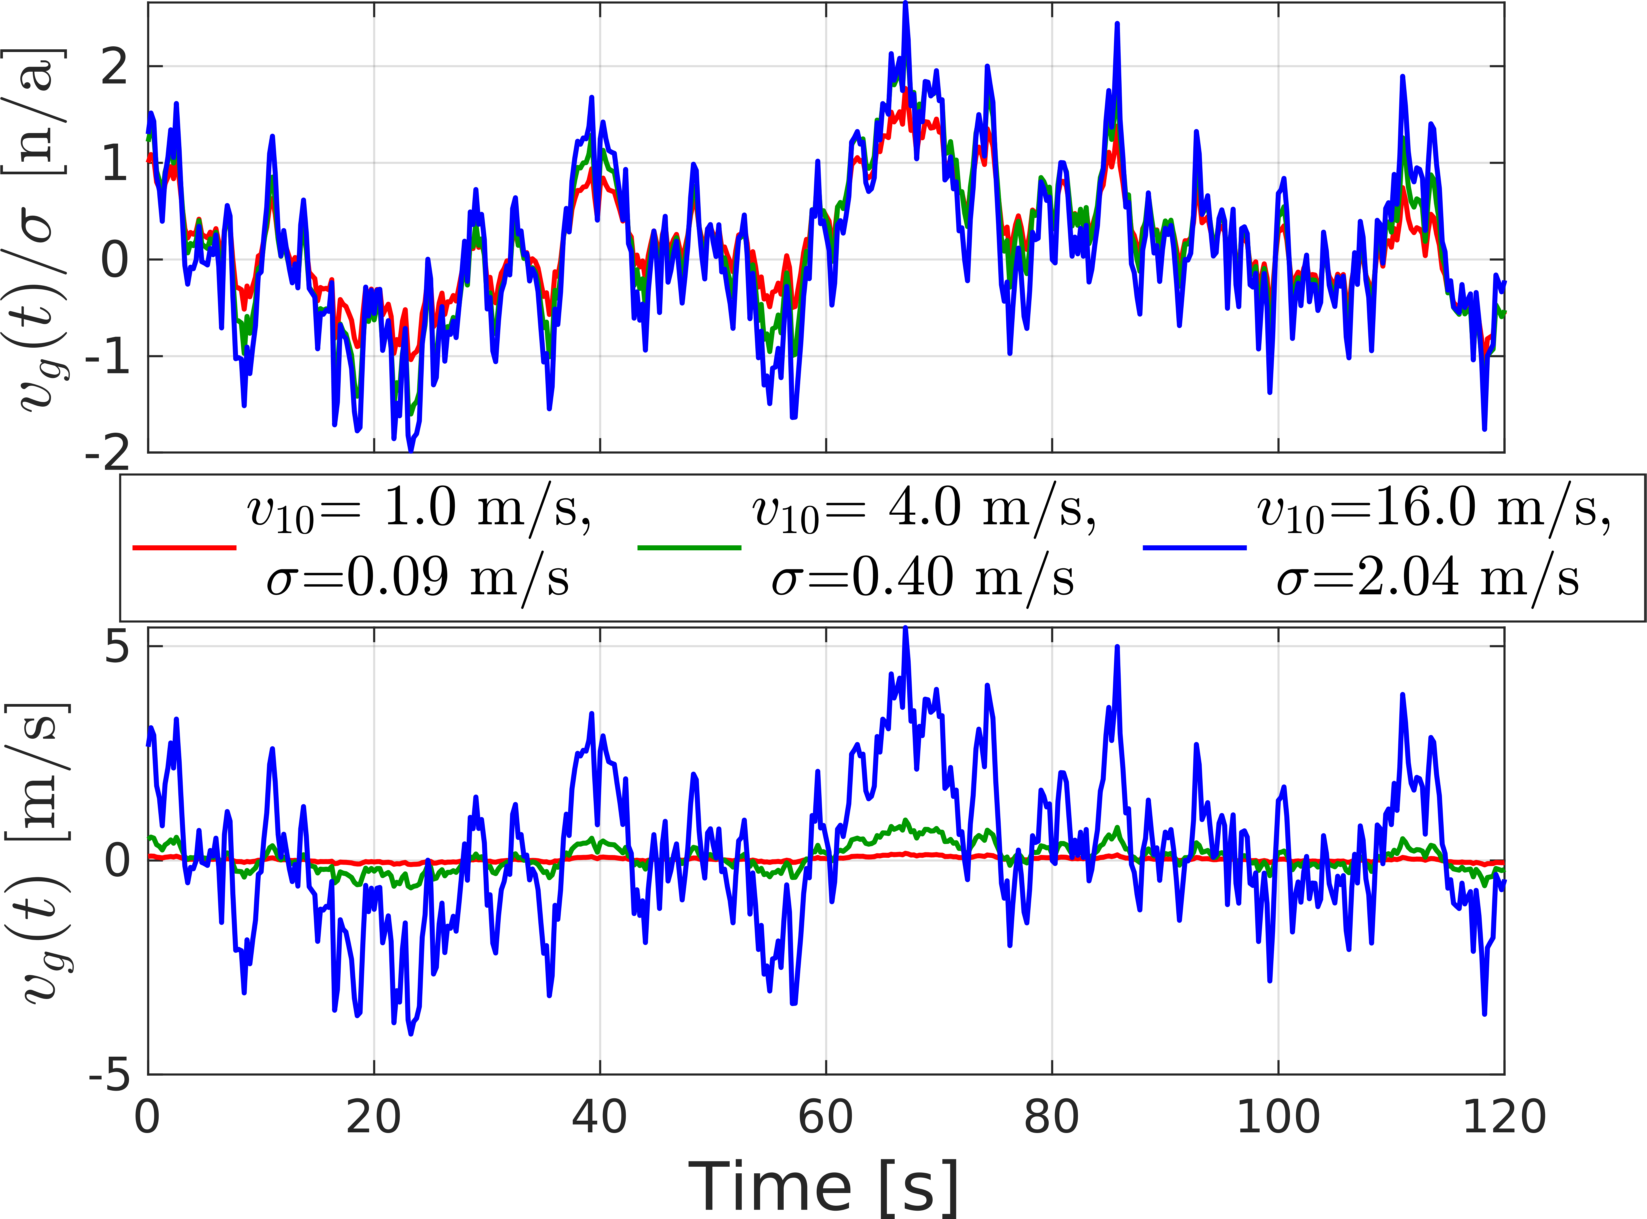
\includegraphics[width=\SFc\textwidth]{src/foristall_time_ex.png}
  \caption{Example time series of variable wind speed component generated by spectral representation for Forristall spectrum for different mean wind speed values.}
  \label{f:forristall}
\end{figure}
In the upper axis, the speed is normalized by the standard deviation of the time series to illustrate the similarity in the results. This view also highlights that the higher mean wind velocities generate spectra with a slightly higher cutoff frequency (\ref{e:cutoff}).

\subsection{Wind Forces}
The model used for simulating the wind environment---consisting of horizontal wind speed ($V_w$) and direction ($\beta_w$)---is described in Section~\ref{s:wind_model}.  We consider the influence of this wind on the maneuvering degrees-of-freedom of the model.  We neglect the wind-induced motion in heave, pitch and roll.  While the influence on heave and pitch are typically very small, for certain vessels, under certain conditions, the wind can have an effect on roll.  For such cases the same coefficient-based model presented below can be extended.

We adapt the model and notation described by \citet{fossen94guidance}.  The relative (apparent) wind velocities are
\begin{IEEEeqnarray}{rCl}\IEEEyesnumber\label{e:relwind}
u_{rw} & = u - u_w \IEEEyessubnumber \\
v_{rw} & = v - v_w \IEEEyessubnumber 
\end{IEEEeqnarray}
where $u_w$ and $v_w$ are the x and y components of the simulated wind velocity in the vessel body frame, expressed as
\begin{IEEEeqnarray}{rCl}\IEEEyesnumber\label{e:wvel}
u_w & = V_w \cos(\beta_w - \psi) \IEEEyessubnumber \\
v_w & = V_w \sin(\beta_w - \psi). \IEEEyessubnumber 
\end{IEEEeqnarray}
The surge, sway and yaw components of the wind force vector ($\bm{\tau}_{wind}$ in \eqref{e:fossenmodel}) are dependent upon the apparent wind and the coefficients for each mode.  For symmetrical vessels, these wind coefficients can be considered constant.  Using dimensional wind coefficients $\bar{c}_x$, $\bar{c}_y$ and $\bar{c}_n$ we express the forcing terms as
\begin{IEEEeqnarray}{rCl}\IEEEyesnumber\label{e:wind} 
  X_{wind} &=&\bar{c}_x u_{rw} |u_{rw}| \IEEEyessubnumber \\
  Y_{wind} &=& \bar{c}_y v_{rw} |v_{rw}|\IEEEyessubnumber \\
  N_{wind} &=& -2.0 \bar{c}_n u_{rw} v_{rw}. \IEEEyessubnumber
\end{IEEEeqnarray}

This wind forcing model is implemented as another standalone Gazebo plugin.  At runtime the user specifies the wind characteristics---mean direction and speed---and the vessel-specific wind coefficients in \eqref{e:wind}. The wind speed and direction at simulation time is calculated according to the wind generation model in \eqref{e:sim2}, the components of the apparent wind are calculated in the vessel body-frame and the resulting forces from \eqref{e:wind} are applied to the simulated vessel for inclusion in the next cycle of the physics engine update.

Analogous to the hydrodynamic model, this approach to representing wind-induced forces is generally applicable to surface vessels and a vessel-specific application requires estimation of the wind coefficients.  For the \wamv{} model, wind coefficients have been estimated based on experimental testing \citep{sarda16station}.  We use these numerical values for the \wamv{} for the purposes of the VRX challenge reference implementation.  

\bibliographystyle{unsrtnat} 
\bibliography{../latexlib/bib/bbing_master}

\end{document}


